\documentclass[a4paper,10pt]{scrartcl}
\usepackage[utf8]{inputenc}
\usepackage{graphicx}
\usepackage{float}
\usepackage{listings}
\usepackage[english]{babel}

% Title Page
\title{\project{}: A multi-platform modular test environment.}
\author{Berend van Veenendaal}
\bibliographystyle{plain}
%hieronder wordt de project naam als variabele gedeclareerd
\newcommand{\project}{Codmon-VM}
\newcommand{\CS}{C\nolinebreak\hspace{-.05em}\raisebox{.6ex}{\bf \#}}

\begin{document}
\maketitle

\begin{abstract}
TODO:Abstract
\end{abstract}
\newpage
\section*{Preface}
\label{sec:Preface}
TODO: Preface,acknowledgements
\newpage
\tableofcontents
\newpage

\section{Introduction}
\label{sec:Introduction}
This chapter introduces the \project{} project by giving a brief description of background of my research and of the
previous version of the Codmon project. It also describes the structure of this thesis.

\subsection{Background}
\label{sec:Background}
In times when software projects become more and more complex, testing of this software becomes more and more important. Many software related problems are caused by lack of testing of the 
software~\cite{TTCST}. Most of the times software testers only test software on one platform. For instance only on a Linux or a Windows platform. Setting-up and configuring again and again all 
the different test environments on different platforms simply costs too much time. So one of the challenges of software testing is to make sure that the software behaves in the same way on 
different platforms, without spending too much time on the installation and configuration of the test environment on all these platforms. Even when the test environment is written in such a way 
that it is able to run on different platforms, there are still issues that must be dealt with, before one is able to run and test the software. So in an ideal world we can test the software without being 
worried about setting up the test environment. 

\subsection{Problem indication}
\label{subsec:Problemindication}
Nowdays there are numerous test frameworks and test environments available. For example there is \emph{Junit}\cite{Junit} for Java-unit testing and \emph{NUnit}\cite{Nunit} for \CS{}-unit testing.
There are also different environments like Hudson\cite{HudsonDoc}\cite{Hudson}, Jenkins\cite{JenkinsDoc} which can build a project and run a series of (unit) tests against this project. 
These frameworks and environments have both their advantages and disadvantages. One of the advantages of unit testing is that a software developer can easily add new \emph{functional} unit tests.
One of the disadvantages is that standard unit testing ignores non-functional tests like performance testing and the deployment of the software. Jenkins and Hudson,like Unit tests, also have their
disadvantages. For instance, although they both run on several platforms, in their usage they are not really platform independent. For example, if you want
to make a connection from Hudson or Jenkins to a remote machine you do this by executing a shell script, so a user must know in advance on which platform this script has to run.
So although it is possible to connect to different machines it is not a 100\% platform independent environment.
 
\subsection{Problem statement}
\label{subsec:Problemstatement}
The test frameworks and test environments mentioned in section \ref{subsec:Problemindication} can be criticized on one or more aspects. What we are looking for is in fact, a combination
of the positive aspects of the described frameworks and environments, without the undesirable aspects. So the central question is, is it possible to design a
multi-platform, modular test environment? In addition, we study if it is possible to design the test environment in a \emph{user friendly} way, meaning that it must
be possible to easily add both new test cases and software without knowing anything about the internal mechanisms of the test environment.\\

\noindent This thesis describes a multi-platform, user friendly modular test environment called \project{}. The \project{} project provides users with a set of virtual machines,
in which Codmon is already installed and preconfigured. The purpose of the virtual machines is to make it easy for users to test software in several environments.  When a user wants to 
test his software on Windows 7, he should download the \project{} windows 7 VM and install it in VM-ware or Virtual box. The same applies for testing his software in an Ubuntu environment. 
By doing it this way the  only tasks a user of \project{} has to do are 1) add their project to an initialization file and 2) add the tests to a so called wrapper file. This will be discussed 
in more detail in section \ref{sec:Codmon2.0}.


\subsection{Thesis outline}
\label{subsec:Thesisoutline}
Section \ref{sec:codmon} first describes the original Codmon framework and why it was built. It also identifies the problems it has. In section \ref{sec:road}, \emph{The road to \project{}}, 
we explain how we got to the final \project{} design. Section \ref{sec:Codmon2.0} describes the implementation of the \project{} project. 
It starts with a general description of the project followed by a detailed explanation of the different modules of \project{}. After this we will evaluate the choices and their consequences 
in section \ref{sec:evaluation}. In Section \ref{sec:conclusion} we discuss the results based on section \ref{sec:evaluation}. We end this section with a brief discussion of related work.

\newpage
\section{Codmon}
\label{sec:codmon}
In this section we describe the original Codmon framework and its shortcomings. The original Codmon framework was built in 2005 by François Lesuer\cite{Codmon}. Originally Codmon was built for 
testing and performance monitoring Ibis projects\cite{Ibis}\cite{Satin}\cite{MPJ}\cite{IPL}\cite{GMI} on the DAS-2\cite{das2} computer. Codmon was able to perform both functional and performance tests. 
\footnote{At this moment both the das2 and Codmon aren't in use anymore.} If for some reason a particular test failed, Codmon raised an alarm and reported the failures. Codmon does this by 
sending an email directly to the programmer who made the last changes in the software that was tested. Codmon also reported in the same way in case the performance drops below a certain threshold. 
Next to sending an email in case of failing tests, Codmon also marks them on a results web page. It was also the intention that Codmon would be extensible. In this the Codmon programmers 
succeeded only partially. We will discuss this more in depth in section \ref{subsec:CodmonProblems}.  

\subsection{The working of Codmon}
\label{subsec:CodmonDesign}
In this section we will describe the design of the Codmon framework. The Codmon framework is more or less modular and consists of a two parts. The first part is the actual Codmon program. This part 
is responsible for a few things, which we will explain in a few minutes. When a user wants to test one of the applications mentioned above, the only thing he or she must do is to make sure that the Codmon 
framework is installed on the Das-2. He or she needs to know nothing of the Codmon program, except for how it should be started. This \emph{core-part} of Codmon is responsible for a few things. first
it creates a \emph{shot} of the actual state of the of the programs that are tested. It does this by executing a set of \emph{sensors} and collecting the output of these executions. later in this 
section we'll explain what sensors are. In case of a performance tests, the sensor file will make the distinction between functional test and performance tests, the test information is stored in 
a RRD database\cite{RRD}. From this data averages are calculated and eventually the graphs are generated\cite{Codmon}. The results of a performance test will be compared with the results of previous tests 
and if the performance result of a test drops below a certain threshold, an alarm is raised. When an alarm is raised, an email is sent to the last contributor of the code of which a test fails. 
The same happens when one or more functional tests are failing.\\

\noindent The second part of the Codmon framework are the sensor files. A sensor file describes a "test set" that can be executed by the Codmon program. Such a sensor file consists of two parts. 
First there is the \emph{onoff} part, which is used for compilation parts and the functional tests.  Second there is the \emph{graph} part. This part is used for the performance tests. 
The core of each sensor element in a sensor file is the CMD attribute. This CMD attribute consists of two basic parts: a wrapper and a shell-script command. This shell-script command can be anything. 
For instance it can be a SVN command, or a ANT job or something else. Listing \ref{list:sensor} gives an example of such a senor. \\

\lstset{
  captionpos=b,
  caption = \emph{Sensor example},
  label =list:sensor
}
\begin{lstlisting}
 <sensor id="update_ok" 
    name="CVS update" 
    cmd="perl CODMON_HOME/codmon/wrappers/time_wrapper.pl 
    CODMON_HOME sh codmon/local/cvsup.sh" 
    scope="ibis" 
    scheduled="false" 
    graph="true" 
    fatal="true" />
\end{lstlisting}
 
\noindent In this case the CMD attribute apparently consists of a wrapper called \emph{time\_wrapper.pl} and a shell-script command called \emph{cvsup.sh}. The wrapper indicates the kind of test
that is executed. The shell-script command indicates which program is tested. In case of Listing \ref{list:sensor} the update time of the CVS repository is is measured.\\


\noindent Where a \emph{sensor} describes the structure of a set of tests, a so called \emph{wrapper} describes the actual test. Wrappers are small programs that are written int the PERL
language. The return value of a wrapper indicates if a test was successful or not. In case of a failure an alarm is raised and both the return value and the actual error code will be mailed to
the programmer who made the last contribution to the code. The results of the performance tests are plotted in a graph, which makes it easy for the developers to see the performance
behavior. It is fundamental to understand that a \emph{wrapper} is not part of the Codmon program itself. Leaving the wrappers outside of Codmon gives a user the possibility to add their own 
wrappers as well as using general wrappers without knowing the the details of the actual Codmon program. A general wrapper is a wrapper that can be used for each software component. The 
\emph{time\_wrapper} is a good example of a general wrapper. Figure 1 shows a schematic picture of the Codmon structure \cite{Codmon}. More technical details about the Codmon implementation 
can be found in \cite{Codmon}.

\begin{figure}[!ht]
  \caption{\emph{figure 1: Codmon}}
  \centering
    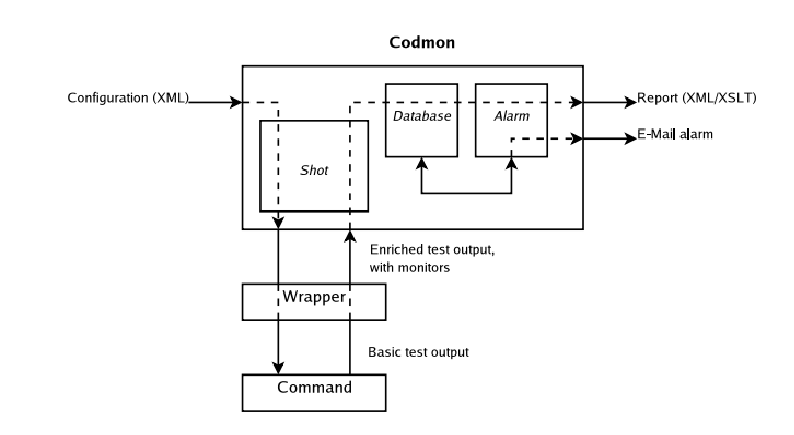
\includegraphics[scale=0.5]{codmon}
\end{figure}



\subsection{Codmon problems}
\label{subsec:CodmonProblems}
The goal of this research was to see if it's possible to design a multi-platform, user friendly modular test environment. There are multiple reasons why Codmon doesn't fit the bill. In this section
we'll discuss these reasons in detail.
 
\subsubsection{Multi-platform}
\label{prob:multi}
First Codmon is not multi-platform. To be multi-platform, without applying every change multiple times, the platform itself must be written in a platform-independent language. 
In Codmon at least three different languages are used. The Codmon program itself is written in Java, which is indeed platform independent\cite{Java}, so this is not the real problem. As we've explained in 
section \ref{subsec:CodmonDesign} the core-part of the sensors is a combination of a \emph{shell-script} command and a \emph{wrapper}. Since a Linux shell-script usually won't work on a Windows environment 
this part is definitely not platform independent. The same can be said about the PERL language, this will without special effort, also not work on a Windows environment. Next to this there are also several 
separate shell-scripts for example, for  CVS-checkouts and the startup of the Codmon framework. Taking this into account, we can easily see that the Codmon framework is far from platform independent.

\subsubsection{Modularity}
\label{prob:modular} 
The second one is the modularity of Codmon. Due to the chaos of different scripts and languages it is difficult for programmers to add new modules or tests to the Codmon framework. Adding new tests and modules 
should be straight forward 

\subsubsection{User-friendliness}
\label{prob:user}
The third reason is the user-friendliness of Codmon. Next to modularity, which also contributes to the user-friendliness of the test environment, Codmon requires quite a bit of configuration,of 
which you don't want to bother anyone, before a user is able to use it. In the reminder of this thesis we'll explain in detail how we have solved these and other issues in the \project{} environment.\\
 
\noindent Another issue regarding to user-friendliness is the structure of the wrappers. As you could see in section \ref{subsec:CodmonDesign} the CMD attribute of a sensor consists of two basic parts: 
a wrapper and a shell-script command, of which the shell-script command could be anything. From a users perspective it would be much easier if there was only one type of command possible, an Ant-job\cite{Ant} 
for instance.

\newpage
\section{The Road to \project{}}
\label{sec:road}
As we described in section \ref{subsec:Problemstatement} our goal is to develop a multi-platform, user friendly modular test environment. This environment must at least satisfy the following requirements. 
The most important requirement is that \project{} is \emph{multiple-platform}. A second requirement is that is should be \emph{modular} and pluggable. This means that it is possible for both users to easily 
add new components to the environment. The same should apply to developers who maintain the environment. A third requirement is that \project{} environment must be user friendly. We don't want to bother 
the users of the \project{} environment with the internal mechanisms of it. A second issue regarding to user-friendliness is that the sensors as described in section \ref{subsec:CodmonDesign} should all 
have the same structure so a user can add tests always in the same way.\\

\subsection{General decisions}
\label{subsec:general}
In the previous sections we have stated that Codmon has some good aspects as well as some aspects that aren't that good. To design a test environment which satisfies the mentioned requirements 
we decided to reuse the good parts of Codmon and design new components where necessary. Since the core program of Codmon is written in Java and Java is multi-platform we decided to reuse most of this code 
and only adapt it if there is no other option. In section \ref{sec:Codmon2.0} we'll show where, how and why we've adapted the Codmon core program. 

\subsection{Multi-platform}
\label{road:multi}
Because the Codmon core program is written in Java already we've decided to write the all wrappers in Java as well. Using as few languages as possible will help the people who have to maintain the 
environment. We also saw that the core of a sensor consists of two parts a wrapper and a shell-script command. In most cases this shell script command will start some program. This program should also 
be able to run on multiple platforms. As we discussed above in \project{} all the wrappers will be written in Java. Hereby writing these programs in Java as well is an obvious choice. So now we have a Java wrapper
and a Java program. We thus need a platform independent construction that, at least, is able to start a program. We have chosen to use \emph{Ant} for this. One of the reasons to choose Ant is that it provides 
us with a lot of flexibility. Lets take a look at the following example. A user who wants to test a piece of Java software probably already has a build file for building the software. So there is nothing new 
here. The only thing the user has to add is a new ant-target, which starts the program. Listing \ref{list:sensorNew} shows the new sensor structure:

\lstset{
  captionpos=b,
  caption = \emph{Sensor new structure},
  label =list:sensorNew
}
\begin{lstlisting}
 <sensor id="update_ok" 
    name="CVS update" 
    cmd="java <wrapper> <path to build file > <ant> <target>" 
    scope="ibis" 
    scheduled="false" 
    graph="true" 
    fatal="true" />
\end{lstlisting}

The \textless target\textgreater \ is an optional value. When the target value is left out, Codmon will run the default ant target. In section \ref{sec:Codmon2.0} we'll show how this all is implemented in the 
\project{} environment.\\

\subsection{Modularity}
\label{road:modular}
Another problem we discussed in section \ref{subsec:CodmonDesign} is the modularity of the environment. The way Codmon was designed it could only handle CVS-checkouts and updates. The \project{} 
environment must be able to deal with different versioning systems. To achieve this we decided to design separate \emph{modules} outside of the \project{} core program that takes care of the checkouts and updates of the 
software that the users want to test. Each of these modules implement the interface for a different version-control system. Adding support for a new version-control system implies that the codmon developers 
(or the users of \project{}) have to write a new module that implements this interface for this new version-control system. This interface should at least define mechanisms for fetching and updating the 
software. Next to this is must also provide some basic mechanism which provide the users with the history log of the software. The only thing a user has to do, is indicate which version control system his 
software is using. We discuss the implementation in more depth in section \ref{sec:Codmon2.0}.\\

\noindent The new sensor structure as discussed in section \ref{road:multi} makes adding new test also straight forward. The only thing a \project{} user has to do is add a new test, and create an Ant target 
for this test. 

\subsection{User-friendliness}
\label{road:user}
When a user wants to test his software on multiple platforms you don't want to download, install and configure the test environment over and over. The \project{} project comes up with a nice and powerful 
solution for this problem. It provides a set of virtual machines in which \project{} is already installed en pre-configured. The only things a user has to do before he can use the by \project{} supplied tests is
to download one or more of these virtual machines, load them into VM-ware and add the details of his software to an initialization file. By doing it this way the nasty configuration details are hidden for the users of the 
\project{} environment. Also when a a new version of an operating system arrives, the \project{} developers only have to configure one new image, which is directly available for all the users. How this works 
exactly we'll see in section \ref{sec:Codmon2.0}. 


\newpage
\section{The implementation of \project{}}
\label{sec:Codmon2.0}
In This section we'll describe how we've implemented the decisions made in section \ref{sec:road} in the \project{} project. We'll discuss the implementation in the same order as the order the different modules 
appear to a user of \project{} environment. When someone wants to use the \project{} test environment there are two options he can choose to get access to this environment. We'll come to these options later in 
this section. For now we assume the user has access to a working \project{} environment.

\subsection{The init.XML file}
\label{subsec:init}

Before the \project{} environment is able to run one or more tests on a software, it has to know where it can find the software and check it out\footnote{for the sake of simplicity,when we talk about it in a 
general way, we call both check-out and clone check-out in this thesis.}. This information and other information has to be added to an \emph{init.xml} file. This file is stored at \emph{"codmon/codmon/local/
checkoutApplications/"}. Listing \ref{list:init} shows the structure of the init file. The explanation of its elements is shown in table \ref{tab:init}. 

\lstset{
  captionpos=b,
  caption = \emph{init.xml example},
  label =list:init
}
\begin{lstlisting}
 <projects>
	<project>
		<name>projectname</name>
		<location>http://www.sampleurl.com</location>
		<versionControl>
			<type>svn</type>
			<command>checkout</command>
		</versionControl>
		<run>true</run>
		<user>username</user>
		<pwd>pwd</pwd>
	</project>
<projects>
\end{lstlisting}  

\begin{table}
\centering
  \begin{tabular}{ | l| p{5cm} |}
  \hline
  \textbf{projects} & List of all the projects that are involved in a test series. \\ \hline
  \textbf{project} & Contains the information of one specific project. \\ \hline
  \textbf{name} & The name of the project. \\ \hline
  \textbf{location} & The URL of the location where the project can be found. \\ \hline
  \textbf{versionControl} & Element that contains specific information about the version-control system \\ \hline
  \textbf{type} & The type of version control system that is used for the project. e.g. \emph{SVN} or \emph{Git} \\ \hline
  \textbf{run} & \textbf{Boolean} that indicates is a project should be tested. \\ \hline
  \textbf{user} & username to login into the version-control system \\ \hline
  \textbf{pwd} & password to login into the version-control system \\ \hline
  \end{tabular}
\caption{Table1 : init.xml elements}
\label{tab:init}
\end{table}



\subsection{wrappers}
\label{subsec:wrappers}

\subsection{Version control}
\label{subsec:versionControl}


\newpage
\section{evaluation}
\label{sec:evaluation}
TODO: This section evaluates the choices that are made in the previous sections'

\newpage
\section{Conclusion and related work}
\label{sec:conclusion}
TODO: give answers to the questions from section Problem statement
TODO: Discus related and future work
\newpage

\bibliography{Master}
\end{document}    